\documentclass[11pt]{beamer}

\usetheme{metropolis}

\usepackage{graphicx}
\usepackage{physics}
\usepackage{adjustbox}
\usepackage{caption}
\usepackage{chemformula}
\usepackage{quoting}
\usepackage[style=chem-angew,backend=bibtex]{biblatex}
\bibliography{references}
%
% Choose how your presentation looks.
%
% For more themes, color themes and font themes, see:
% http://deic.uab.es/~iblanes/beamer_gallery/index_by_theme.html
%
\mode<presentation>
{
  \usetheme{default}      % or try Darmstadt, Madrid, Warsaw, ...
  \usecolortheme{default} % or try albatross, beaver, crane, ...
  \usefonttheme{default}  % or try serif, structurebold, ...
  \setbeamertemplate{navigation symbols}{}
  \setbeamertemplate{caption}[numbered]
  \setbeamerfont{footnote}{size=\tiny}
} 

\usepackage[english]{babel}
\usepackage[utf8]{inputenc}
\graphicspath{{image/}}

\AtBeginSection[]{
\begin{frame}{Outline}
  \tableofcontents[currentsection]
\end{frame}
}

\title{Chapter 8: Chemical Bonding}
\institute{Chemistry Department, Cypress College}
\date{Nov 9, 2022}

\begin{document}

\begin{frame}
  \titlepage
\end{frame}

\begin{frame}{Class Announcements}
  \textbf{Lab}
  \begin{itemize}
  \item Experiment 17 Lewis Structures and Molecular Models
  \item Basic steps for lewis structures
  \item Reminder - Need $70\%$ of laborator points to pass
    the course
  \end{itemize}

  \textbf{Lecture}
  \begin{itemize}
  \item Finish up Ch 7 and begin Ch 8
  \item Go over homework 9 (EC for students who present)
  \item Quiz and Homework assignment released Fri, Nov 11th at 3pm
  \end{itemize}
\end{frame}

\section{Review: Electron Configuration of Ions}

\begin{frame}{Principles for Filling Atomic Orbitals}
  \textbf{Aufbau principle} - electrons fill an orbital starting with
  the lowest energy level

  \textbf{Pauli exclusion princple} - No two electrons with the same
  spin can occupy the same orbital

  \textbf{Hund's Rule} - Maximize the number of unpaired electrons
\end{frame}

\begin{frame}{Electron Configurations of Ions}
  \textbf{Cations} - Remove electrons from the highest energy atomic
  orbitals

  \textbf{Anions} - Follow the same Aufbau principle by filling orbitals
  with the lowest energy level

  \onslide<2->{\textbf{Q:} For transition metals, which atomic orbitals, s or d,
    do you begin removing electrons from?
  }
\end{frame}

\begin{frame}{Orbital Diagram - Multielectron Element}
  \textbf{Q:} These diagrams show the relative energies of unfilled orbitals.
  Based on these orderings, do the relative energies of completely filled orbitals hold true?
  
  \centering
  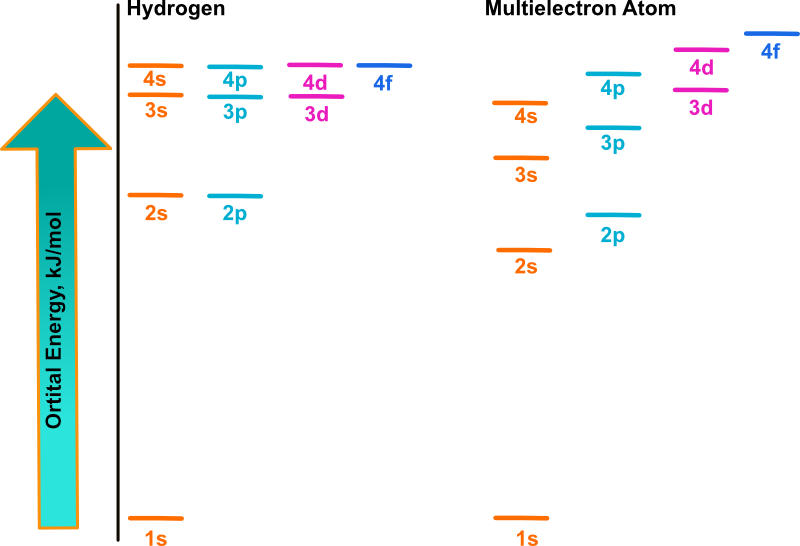
\includegraphics[scale=1.3]{orbital_energy}
\end{frame}

\section{Types of Bonds}

\begin{frame}{Water is Life}
  \centering
  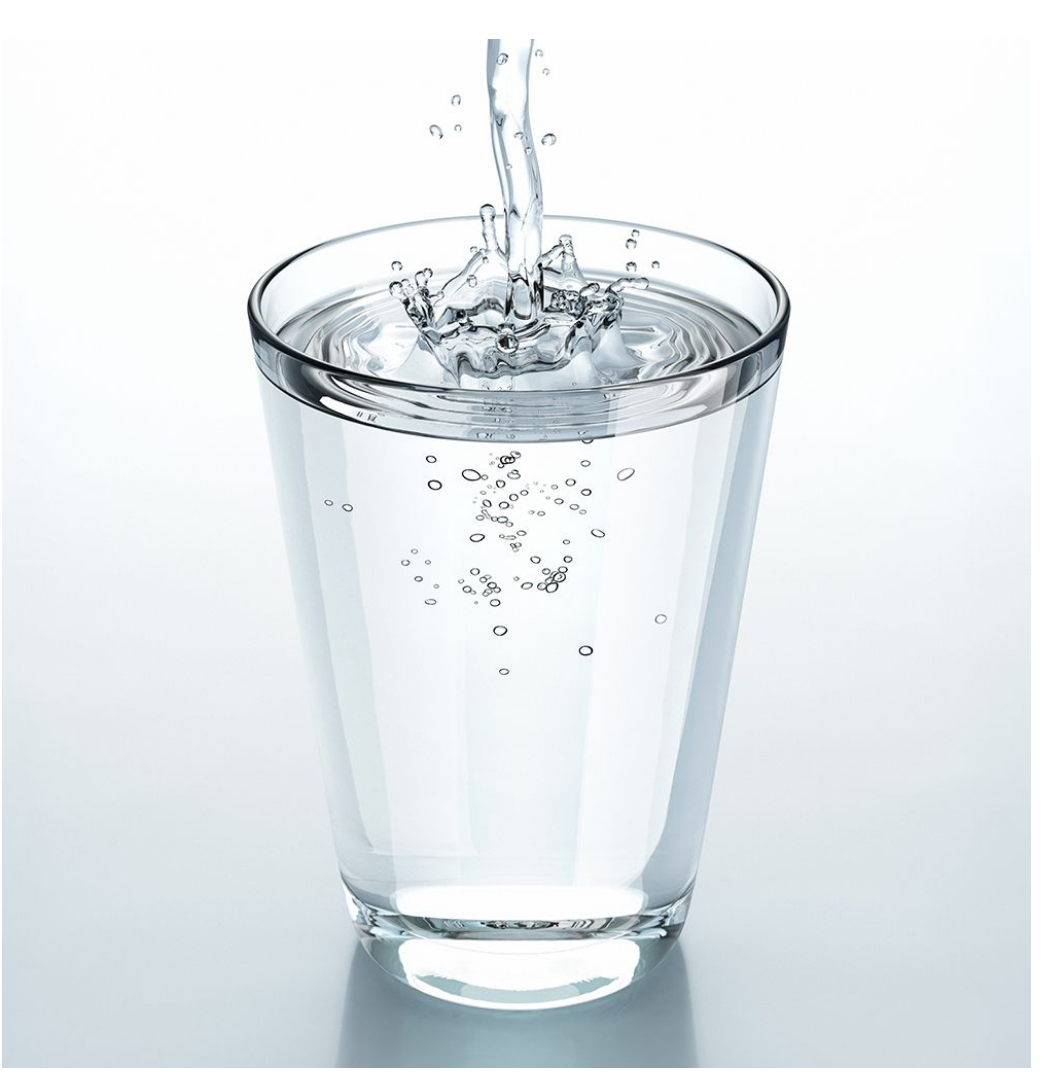
\includegraphics[width=0.4\linewidth]{water}
  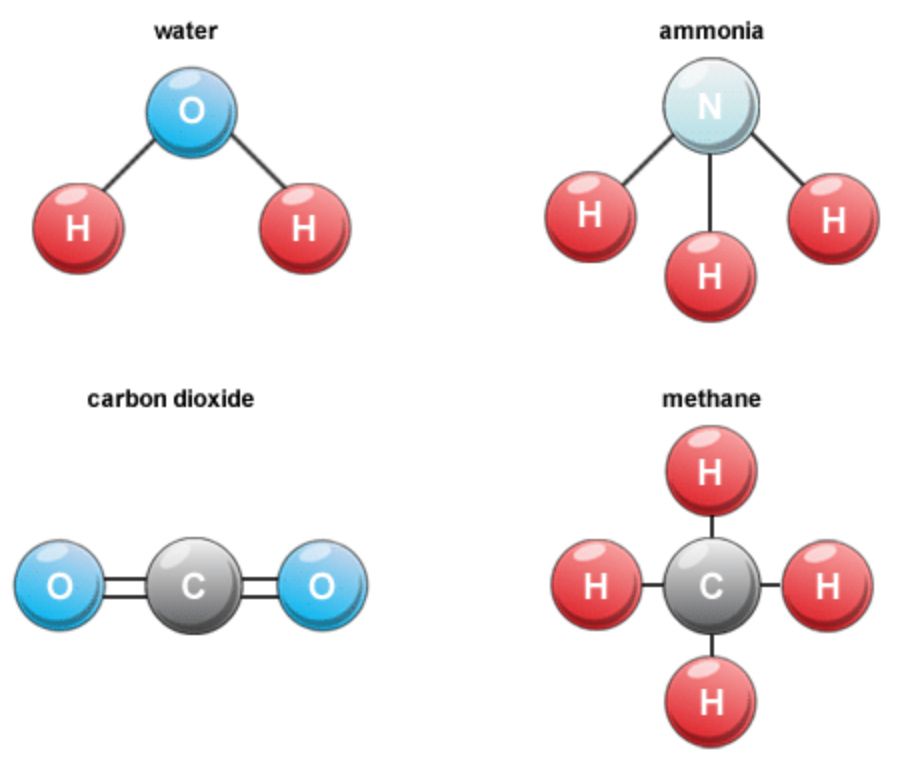
\includegraphics[width=0.4\linewidth,trim={0 6in 7in 0},clip]{molec_example}

  \begin{itemize}
  \item Liquid water made up of moles upon moles of water molecules
  \item Molecules are made up of atoms connected by ``chemical bonds''
  \end{itemize}
\end{frame}

\begin{frame}{What are Chemical Bonds?}
  \begin{center}
    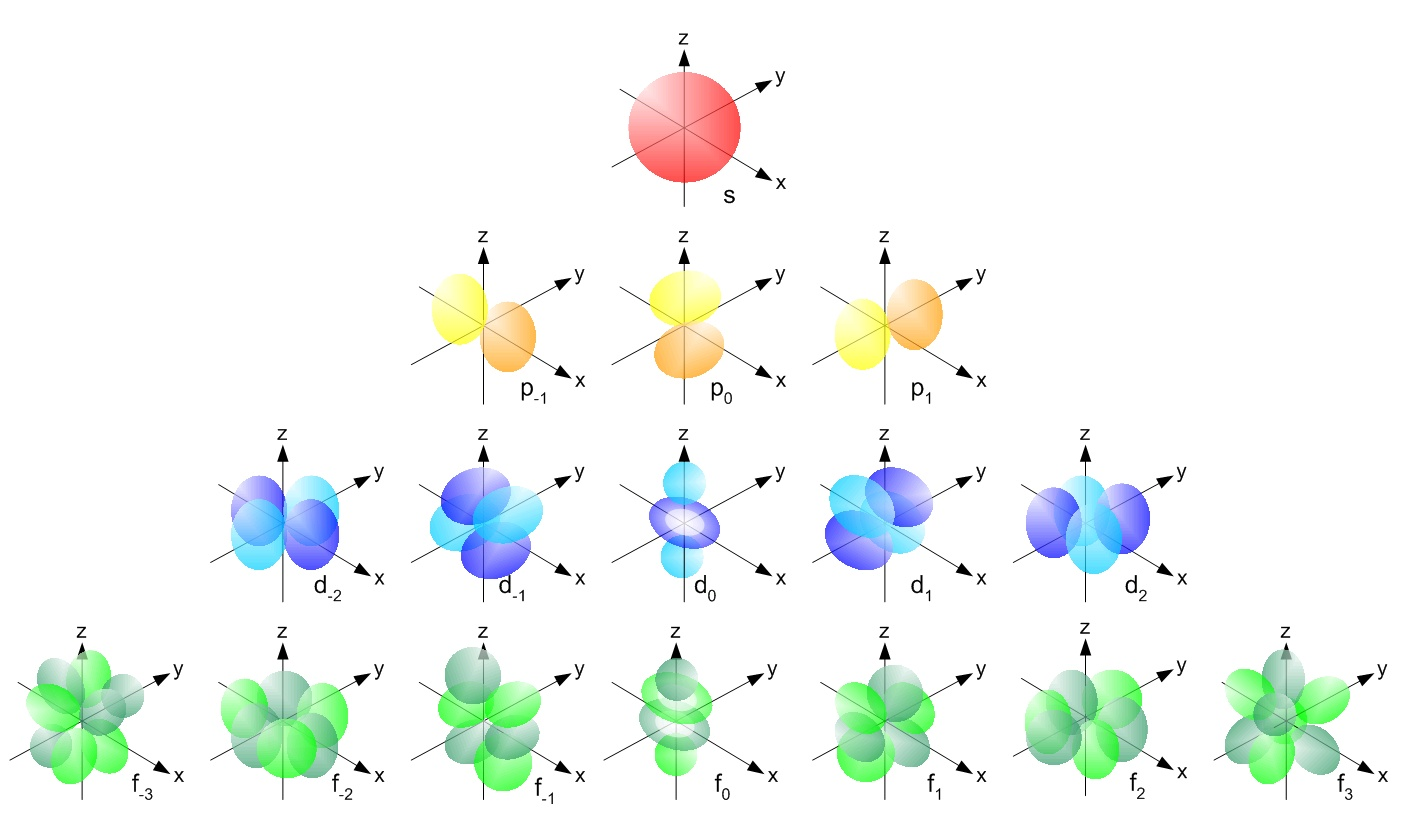
\includegraphics[width=0.8\linewidth]{single_elect_orb}
  \end{center}
  \textbf{Bonds are made up of atomic orbitals}
  \begin{itemize}
  \item Overlap of atomic orbitals lead to the formation of molecular
    orbitals (same energy and specific orientation)
  \end{itemize}
\end{frame}

\begin{frame}{Example of p-orbitals}
  \centering
  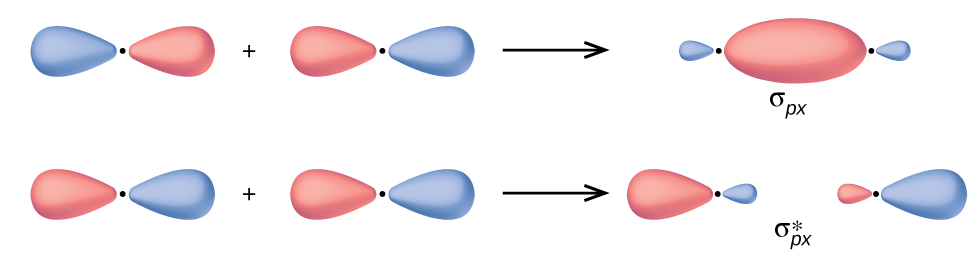
\includegraphics[width=\linewidth]{p_sigma}
  \begin{itemize}
  \item Depending on the orientation, p-orbitals
    will form a bond
  \end{itemize}
\end{frame}

\subsection{Ionic and Covalent Bonds}

\begin{frame}{Ionic Bonds}
  \begin{center}
    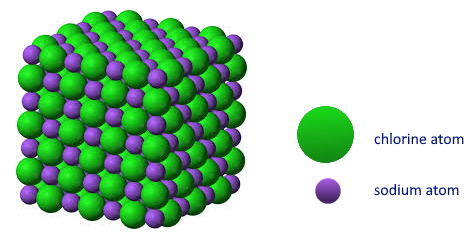
\includegraphics[width=0.6\linewidth]{nacl}
  \end{center}
  
  \textbf{Ionic Compounds} - Made up of cation and anion

  \textbf{Ionic Bonds} - Hold the cations and anions together;
  purely electrostatic interaction

  \onslide<2->{\textbf{Q:} For ionic bond, are the electrons shared
    between the cation and anion?}
\end{frame}

\begin{frame}{Covalent Bonds}
  \begin{center}
    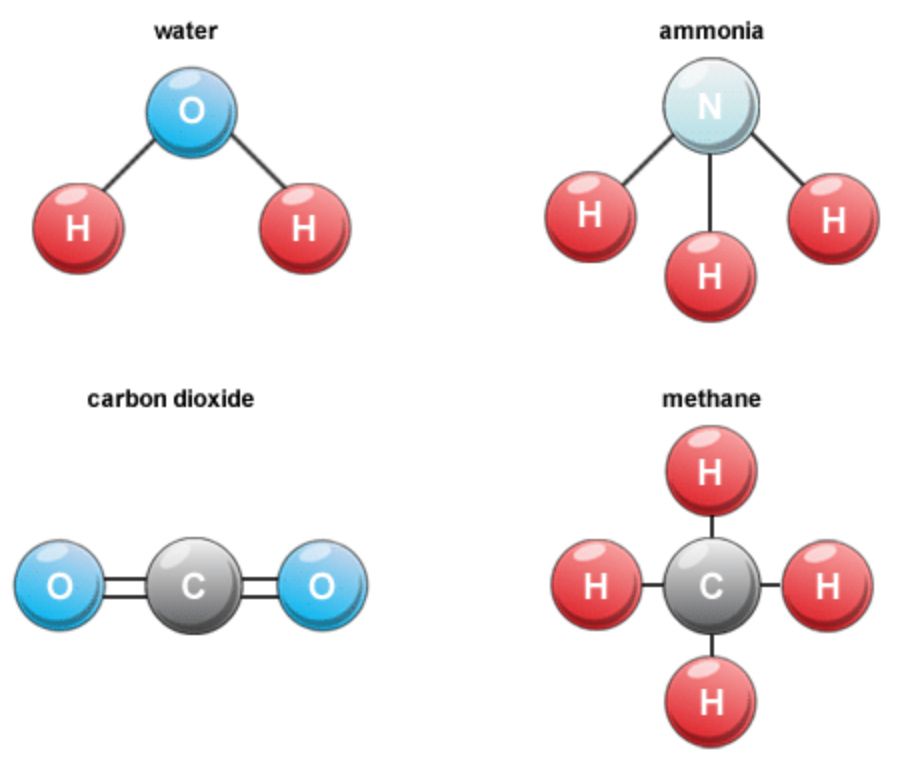
\includegraphics[width=0.6\linewidth]{molec_example}
  \end{center}
  \begin{itemize}
  \item Electrons are shared between atoms to achieve
    the octet rule
  \item \textit{Note:} Octet rule can be broken for atoms
    after the 3rd row e.g. P, S, Cl, etc.
  \end{itemize}
\end{frame}

\subsection{Electronegativity}

\begin{frame}{Electronegativity: Tug-of-War}
  \centering
  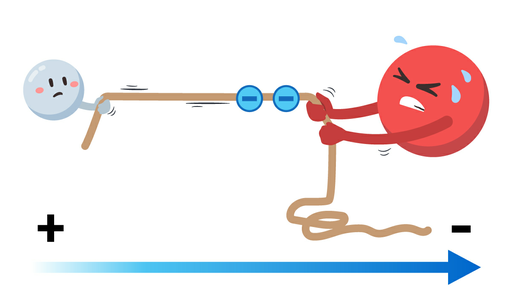
\includegraphics[width=0.8\linewidth]{water_tug}
  \begin{itemize}
  \item Sharing of electrons can lead to unequal pull
    (electronegativity)
  \end{itemize}
\end{frame}

\begin{frame}{Electronegativity Trends}
  \centering
  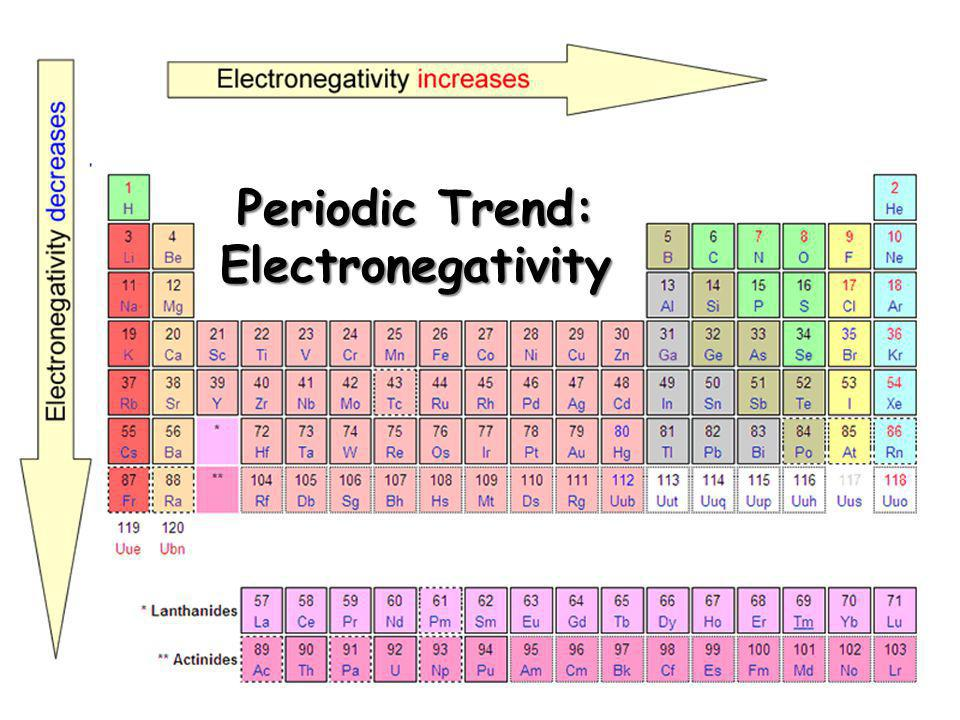
\includegraphics[width=\linewidth]{electronegativity}
\end{frame}

\begin{frame}{Practice: Polarity}
  \textbf{Which of the following is the most polar bond?}

    C--C; C--H; N--H; O--H; F--H; Se--H
\end{frame}

\section{Drawing Lewis Structures}

\begin{frame}{Octet Rule}
  \textbf{Octet Rule} - Atoms have a tendency to achieve
  an electron configuration having 8 valence electrons

  \textbf{Q:} How many electrons are needed for the following
  atoms to achieve the octet rule: C, N, O, F, Xe, and Ne
\end{frame}

\begin{frame}{Exception to Octet Rule}
  \begin{center}
    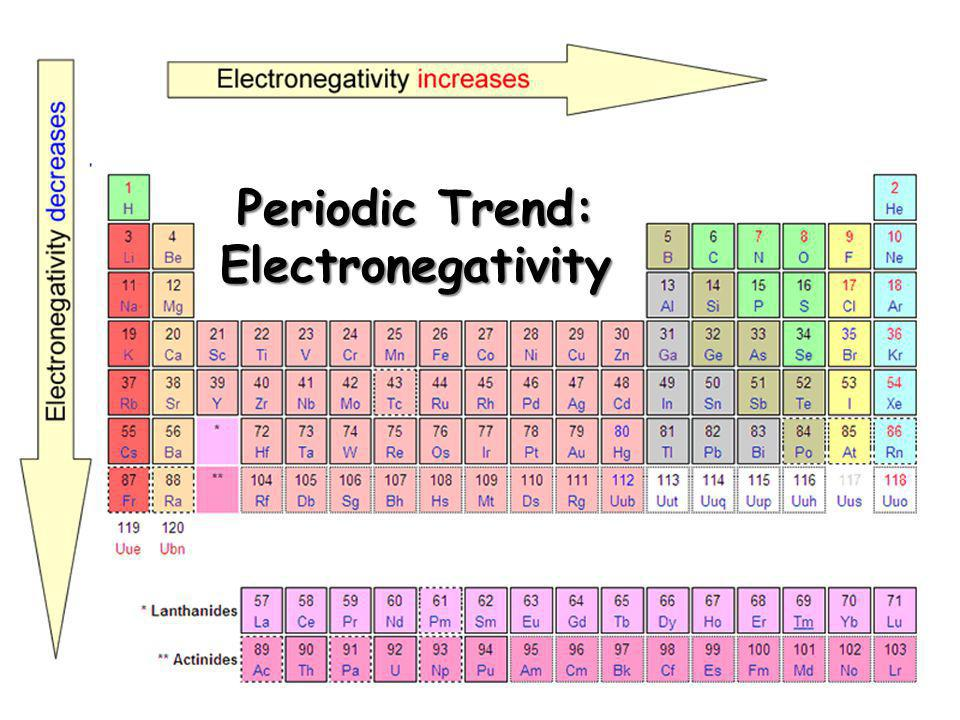
\includegraphics[width=0.75\linewidth]{electronegativity}
  \end{center}
  
  \textit{Exceptions:} Atoms starting in the
    3rd row can break the octet rule

  \onslide<2->{\textbf{Q:} Why are these atoms able to break
    the octet rule?}
\end{frame}

\begin{frame}{Drawing Lewis Structures}
  \begin{enumerate}
  \item Count the total number of valence electrons
  \item Draw the atomic skeleton by determining the central atoms
    (generally the one capable of making many bonds)
  \item Add single bonds (each counts as 2 electrons) to atoms
    and add lone pairs if needed to satisfy the octet rule
  \item Check that if the amount of valence electrons counted match
    the Lewis structure
  \item Check formal charges on the atoms
  \end{enumerate}
\end{frame}

\begin{frame}{Computing Formal Charges}
  \begin{center}
    Formal Charge = VE - $\frac{1}{2}$ BE - NBE
  \end{center}
  where VE is the number of valence electrons, BE is the bonding
  electron, and NBE is the nonbonding electron aka lone pairs
\end{frame}

\begin{frame}{Practice: Draw Lewis Structures}
  Draw the Lewis structures and compute the formal charges for the
  following: CO$_2$, CN, HCl, O$_3$, CO$_3^{2-}$
  \vspace{1.75in}
\end{frame}

\begin{frame}{Resonance Structures}
  As seen in the previous slide, O$_3$ and CO$_3^{-2}$ have multiple
  structures that are valid

  \textbf{Resonance structures} - the movement of electrons satisfying
  a valid Lewis Structure
  
  \centering
  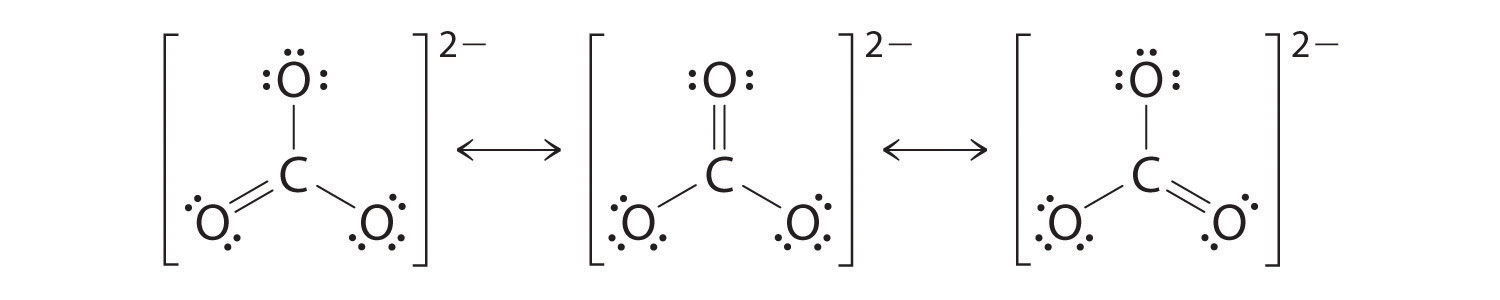
\includegraphics[width=1\linewidth]{resonance_struct}
\end{frame}

\begin{frame}{Practice: Drawing Resonance Structures}
  Draw the resonance structures and resonance hybrid for the following:

  HCO$_2^{-}$, NO$_2^-$, SO$_2$, CNS$^-$, and N$_2$O
  \vspace{1.75in}
\end{frame}

\begin{frame}{Functional Groups in Hydrocarbons}
  \textbf{Functional Groups} - derivatives of a hydrocarbon
  \begin{center}
    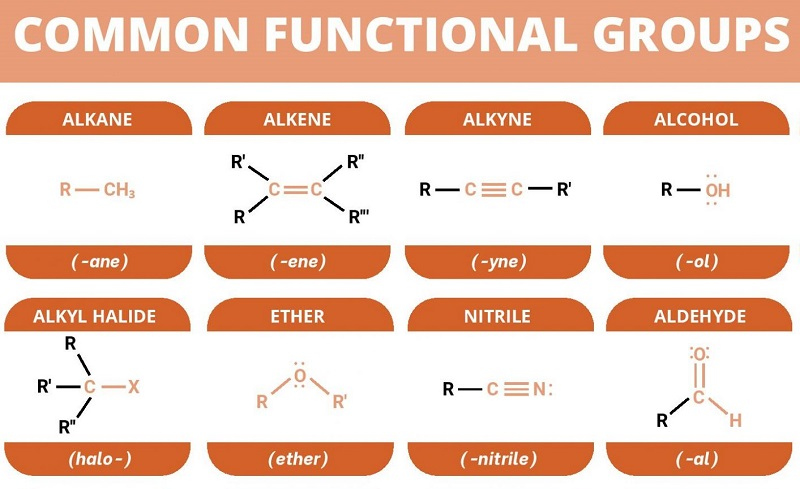
\includegraphics[width=0.8\linewidth]{func_groups}
  \end{center}
  where R represents hydrocarbon component
\end{frame}

\begin{frame}{Practice: Drawing Hydrocarbons}
  Draw the lewis structures for the following hydrocarbons:
  CH$_4$, C$_3$H$_8$, CH$_8$, C$_2$H$_2$
  \vspace{1.75in}
\end{frame}

\section{VSEPR Theory}

\begin{frame}{VSEPR Theory}
  \textbf{VSEPR Theory} - predict the geometric shape of a
  molecule or an ion; minimizes the electronic repulsion of
  the lone pairs
\end{frame}

\begin{frame}
  \vspace{0.15in}
  \centering
  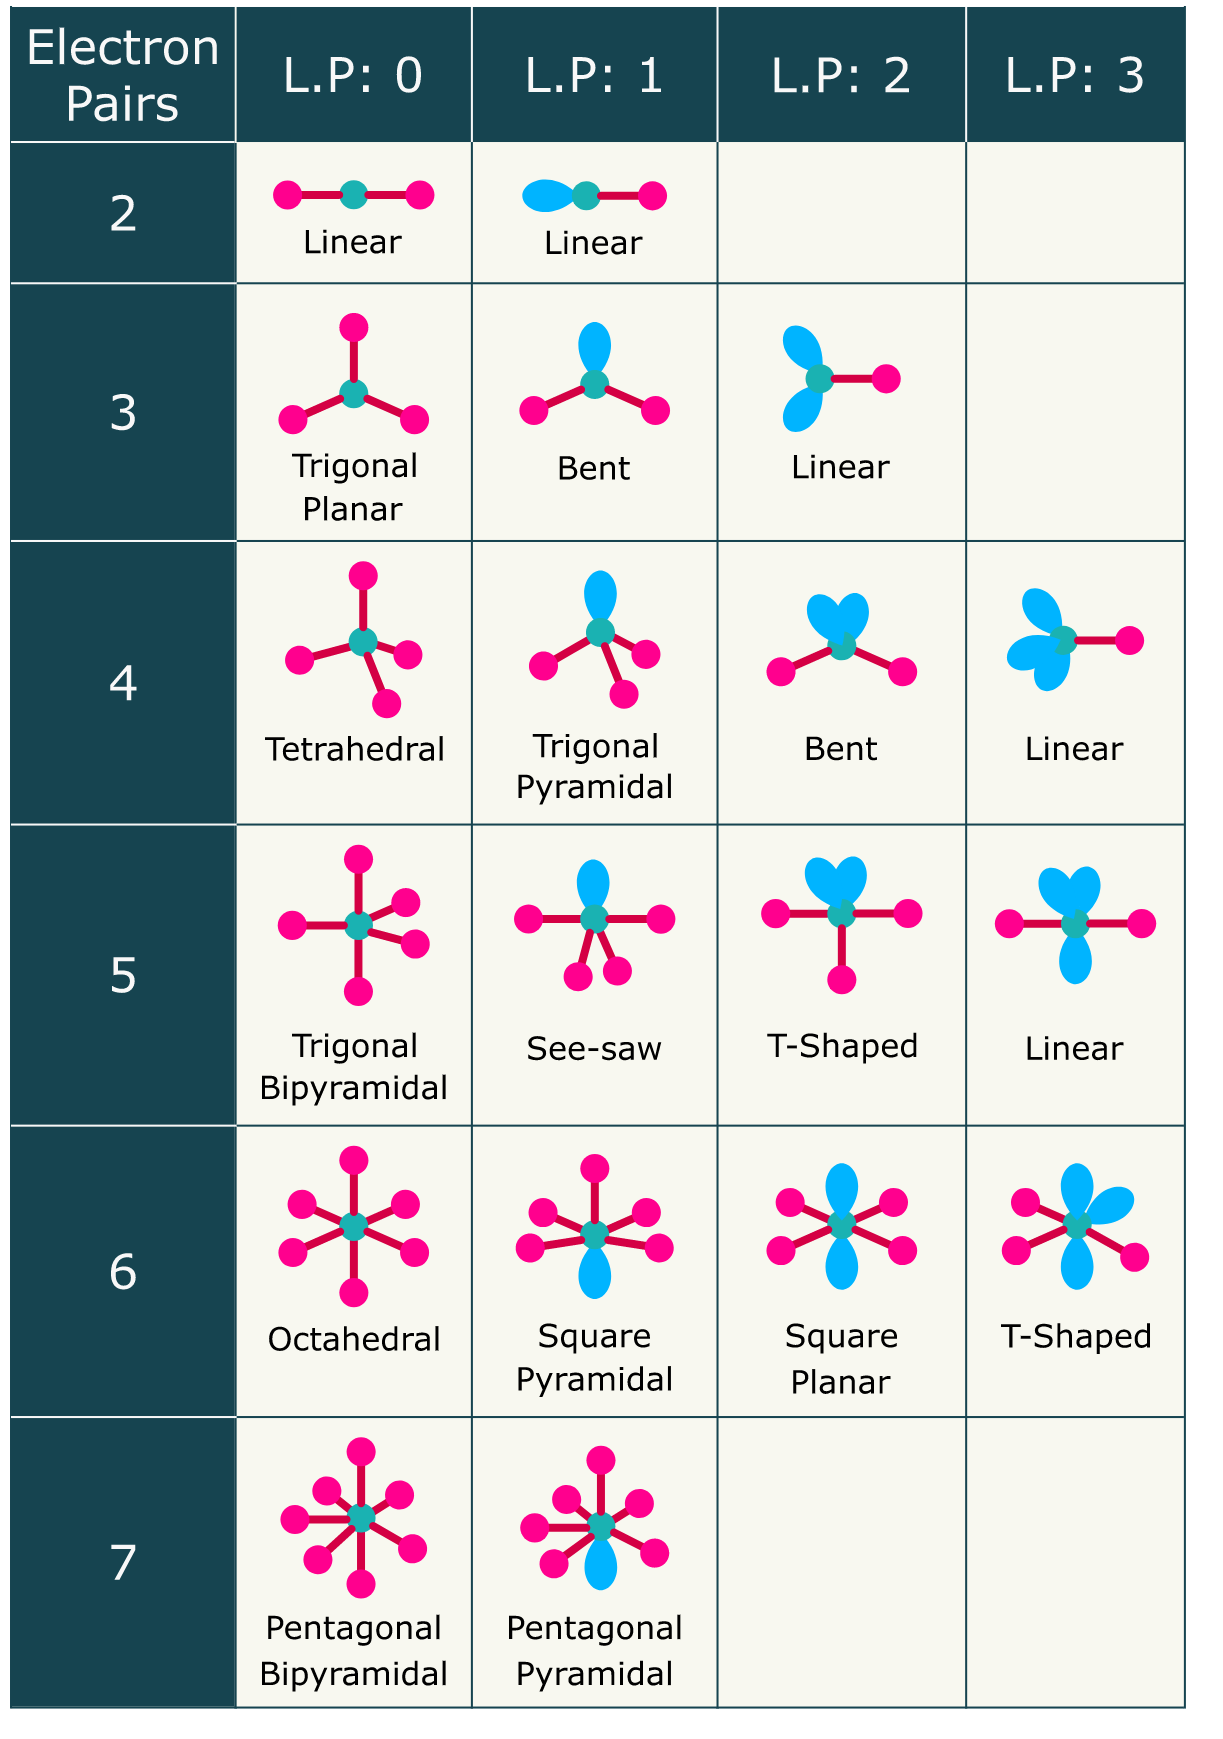
\includegraphics[width=0.6\linewidth]{vsepr_diag}
\end{frame}

\begin{frame}{Practice: Determine the Geometry}
  CO$_2$, CN, HCl, O$_3$, CO$_3^{2-}$,
  CH$_4$, C$_3$H$_8$, CH$_8$, C$_2$H$_2$
  \vspace{1.75in}
\end{frame}

\end{document}
